\chapter{Preliminaries}
\label{chap:num_1}

The chapter is going to provide the introduction to the core concepts of \textit{Semantic Web}, \solid{} and \lpa{} platform. As the concepts explained here will be often referred to in further chapters, it is important to get familiar with them for a complete understanding of every consecutive chapter. 

\section{Semantic Web}

The Semantic Web represents the next significant iteration in connecting data and information over World Wide Web. It adds an ability for a data to be linked from any source to any other source allowing computers to understand the semantics of it and perform increasingly complex computational operation on them. The major idea that makes Semantic Web technology and other data related technologies such as relational databases, is that it focused on preserving the meaning of the data rather than structuring it in efficient manner. 

There are three main technical specifications defining the Semantic Web technologies:
\begin{itemize}
	\item \gls{RDF}, is a data modelling language designed for Semantic Web. Every information in Semantic Web is represented in the RDF.
	\item \gls{SPARQL}, is a query language for Semantic Web. It is mainly designed for querying data across different data sets represented in RDF.
	\item \gls{OWL}, is a knowledge representation language for Semantic Web. It allows defining entities and concepts in a way that allows high reusability for many different applications and purposes.
\end{itemize}  

In other words, the usage of the technology stack mentioned above is what defines a Semantic Web application and differentiates it from any other technologies related to data.

\subsection{RDF}


\section{SOLID}

\section{\lpa{}}

%  TODO : describe components of the architecture

\begin{figure}[h]

\centering
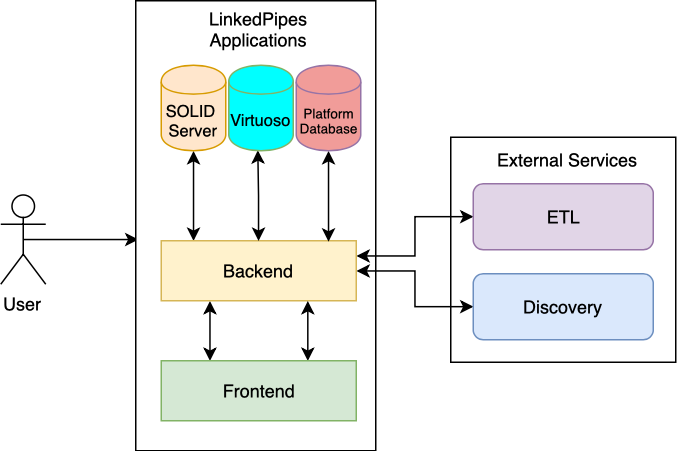
\includegraphics[width=12cm]{lpa_high_level_architecture.png}
\caption{High-level overview of LinkedPipes Applications Platform}
\label{fig:high-level-arch}
\end{figure}

As mentioned in previous chapters, the overall goal of LinkedPipes Applications is to create a web-based tool that would allow generation of interactive visualizations by some domain expert, that can then be embedded in an online article or on another web page or perhaps simply accessed as a standalone page.

The following section uses the various acronyms and terms specific to Semantic Web: 

\begin{itemize}
    \item \gls{IRI} -- IRIs are a superset of Uniform Resource Identifiers (URI) which allow for the inclusion of Unicode characters such as Chinese or Cyrillic symbols in the identifier string. IRIs are extensively used as entity identifiers in Linked data.
    \item SPARQL endpoint is an interface through which a user can query and inspect data stored in a particular RDF data storage.
    \item Dataset is a collection of data available for access or download from a single data store such as a catalog or a SPARQL endpoint.
    \item TTL -- short for Terse RDF Triple Language, one of the RDF serialization formats.
\end{itemize}

\subsection{Components overview}

At the lower level, the \lpa{} is a bundle of various complex services and database solutions communicating between each other in docker environment. 

\begin{figure}[h]
    \centering
    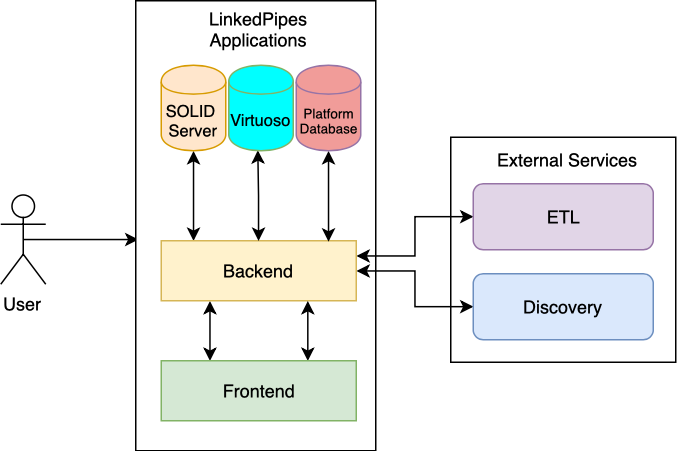
\includegraphics[width=14cm]{lpa_high_level_architecture.png}
    \caption{High-level overview of LinkedPipes Applications Platform}
    \label{fig:lpa-high-level-arch}
\end{figure}

Generally, we can categorize it into three main parts: 

\begin{itemize}
    \item \textbf{\lpa{}} - the main platform from LinkedPipes bundle, and the main stakeholder for \lpas{} project. Combines multiple database solutions for LinkedData, conventional SQL for storing user related records and implementation of a backend and frontend for creating applications.
    \item \textbf{LinkedPipes Services} - a set of external services provided from LinkedPipes bundle that \lpa{} heavily utilizes. Provides a toolset for identifying how linked data can be discovered, extracted, transformed and loaded into an RDF file for further processing.
    \item \textbf{\lpas{}} - the main goal of the following thesis and a functional storage solution for \lpa{} platform. Contains a set of API controllers and managers that allow users of \lpa{} to store and share their applications in a secure and decentralized way. Consecutive chapters will provide a detailed overview of an architecture and implementational details.
\end{itemize}

\subsubsection{Frontend}

\subsubsection{Backend}

\subsubsection{Virtuoso DB}

\subsubsection{PostgreSQL} 

\subsection{LinkedPipes Services} 

\subsubsection{Discovery} 

\subsubsection{ETL} 

% A detailed overview of the solution as well as the overview of current alternatives to \solid is provided in the consecutive chapters of this thesis. 